\section{Stochastische Prozesse}

In einer einführenden Vorlesung zur Stochastik betrachtet man zunächst einzelne Zufallsvariablen, 
etwa das Ergebnis eines Würfelwurfs. In dieser Arbeit stehen hingegen Folgen von 
Zufallsvariablen im Mittelpunkt. Solche Folgen erlauben es, zeitliche Entwicklungen zu modellieren,
beispielsweise Veränderungen eines Systems, die zu bestimmten Zeitpunkten $t_0, t_1, \dots$ gemessen werden.
Man spricht dann von einem zeitdiskreten stochastischen Prozess. Eine natürliche 
Verallgemeinerung bilden zeitstetige stochastische Prozesse: Hierbei definiert man eine 
Familie von Zufallsvariablen $(X_t)_{t \in \mathbb{R}_{\ge 0}}$, wobei $t$ kontinuierlich als 
Zeitparameter interpretiert wird. Ziel dieser Arbeit ist es, Aktienkurse und später Optionswerte mit einem stochastischen Prozess 
zu modellieren.

\begin{bsp}[Zufallsspaziergang]
Ein einfacher stochastischer Prozess ist der \textit{Zufallsspaziergang} (random walk).
Die Position des Spaziergängers zur Zeit $t$ wird durch eine Zufallsvariable $X_t$ beschrieben. 
Man startet bei $X_0 = 0$. In jedem Zeitschritt bewegt sich der Spaziergänger entweder 
einen Schritt nach rechts oder nach links, jeweils mit Wahrscheinlichkeit $p$ bzw. $1-p$. 
Formal gilt:
$$
X_{t+1} = X_t + \xi_{t+1},
$$
wobei $\xi_{t+1}$ eine unabhängige Zufallsvariable ist mit
$$
\xi_{t+1} = 
\begin{cases} 
+1, & \text{mit Wahrscheinlichkeit } p, \\
-1, & \text{mit Wahrscheinlichkeit } 1-p.
\end{cases}
$$

\end{bsp}

\begin{bsp}[Binomialmodell]
Das Binomialmodell ist ein simples Modell einer Aktie und deren Preisentwicklung. 
Man beginnt mit einem Anfangspreis $S_0$. $S_1, S_2, \dots$ sind dann Messungen des Aktienpreises zu einem festen Intervall.
 Zu einer festen Wahrscheinlichkeit $0 \lt p \lt 1$ steigt die Aktie um den Faktor $u$, oder fällt mit der Wahrscheinlichkeit $1-p$ um den Faktor $d$. Also
$$S_{t+1} = \begin{cases} 
    d \cdot S_t, & \text{mit Wahrscheinlichkeit }  p \\ 
    u \cdot S_t, & \text{mit Wahrscheinlichkeit }  1-p

\end{cases}.$$
Im Gegensatz zum Zufallsspaziergang sind die Schritte hier nicht additiv, sondern multiplikativ. Daher
eignet sich das Binomialmodell (im Gegensatz zum Zufallsspaziergang) zur Modellierung von Aktienkursen, es sind keine negativen Preise möglich.

\begin{center}
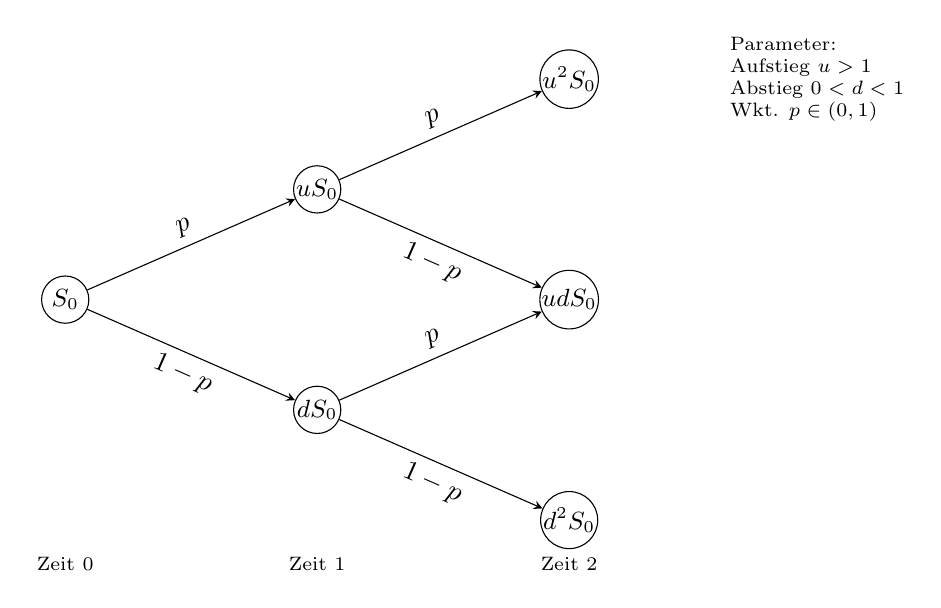
\begin{tikzpicture}[x=3.2cm,y=1.4cm,>=stealth]
    % styles
    \tikzset{price/.style={circle,draw,minimum size=6mm,inner sep=0pt,font=\small}}

    % nodes
    \node[price] (S0)  at (0,0)   {$S_0$};
    \node[price] (Su)  at (1,1)   {$u S_0$};
    \node[price] (Sd)  at (1,-1)  {$d S_0$};
    \node[price] (Suu) at (2,2)   {$u^2 S_0$};
    \node[price] (Sud) at (2,0)   {$u d S_0$};
    \node[price] (Sdd) at (2,-2)  {$d^2 S_0$};

    % edges with probabilities p and 1-p
    \draw[->] (S0) -- node[sloped,above] {$p$} (Su);
    \draw[->] (S0) -- node[sloped,below] {$1-p$} (Sd);

    \draw[->] (Su) -- node[sloped,above] {$p$} (Suu);
    \draw[->] (Su) -- node[sloped,below] {$1-p$} (Sud);

    \draw[->] (Sd) -- node[sloped,above] {$p$} (Sud);
    \draw[->] (Sd) -- node[sloped,below] {$1-p$} (Sdd);

    % time axis labels
    \node[font=\scriptsize] at (0,-2.4) {Zeit 0};
    \node[font=\scriptsize] at (1,-2.4) {Zeit 1};
    \node[font=\scriptsize] at (2,-2.4) {Zeit 2};

    % parameter box
    \node[anchor=west, align=left, font=\scriptsize] at (2.6,2.0) {Parameter:\\
        Aufstieg $u>1$\\
        Abstieg $0<d<1$\\
        Wkt. $p\in(0,1)$
    };
\end{tikzpicture}
\end{center}

\end{bsp}
\begin{bsp}[Brownsche Bewegung]
Die Brownsche Bewegung beschreibt die Bewegung eines Partikels in 
einer Flüssigkeit \cite{webster_bb}. Die Zufallsgröße ist hier die Position des Partikels.
Naturanaloge stochastische Prozesse erfüllen oft eine Stetigkeitsbedingung: 
Andernfalls würde sich z. B. der Partikel in der Flüssigkeit teleportieren. 
Konkret: Es bezeichne der Pfad $t \mapsto X_t$ die Realisierungen der Zufallsvariablen $X_t$ unter 
der Zeit $t$. Dann wird gefordert, dass die Pfade fast-sicher stetig sind, also 
$$P(\{\omega \in \Omega | t \mapsto X_t(\omega) \text{ ist stetig}\}) = 1.$$ 
Im nächsten Kapitel wird die Brownsche Bewegung formal definiert.
\end{bsp}

\subsection{Bedingter Erwartungswert und Filtrationen}

Im Folgenden wird stochastische Unabhängigkeit und der Erwartungswert im Bezug auf die Zeit untersucht. 
Dazu definiert man einen neuen Wahrscheinlichkeitsraum, 
der alle möglichen Verläufe des Prozesses vereint. 
Um nicht weiter zwischen zeit-stetigen und -diskreten Prozessen unterscheiden zu müssen, 
sei $I = \Bbb N_0$ im diskreten und $I = \Bbb R_{\ge 0}$ im stetigen Fall. 
Des weiteren sei $(\tilde \Omega, \mathcal A_t, \tilde P)$ ein Wahrscheinlichkeitsraum, 
und $(X_t)_{t \in I}$ ein eine Familie von Zufallsvariablen auf dem Wahrscheinlichkeitsraum, 
die einen stochastischen Prozess bilden. Vorerst wird der Prozess 
auf dem Produkt-Wahrscheinlichkeitsraum
$$(\Omega, \mathcal F, P) := \bigtimes_{t \in I}(\tilde \Omega, \mathcal A_t,\tilde P)$$
betrachtet.

\begin{defi}[Adaptiertheit]
In der modernen Wahrscheinlichkeitsrechnung wird Information über den
Wahrscheinlichkeitsraum $(\Omega, \mathcal F, P)$ als Teil-$\sigma$-Algebra 
von $\mathcal A$ verschlüsselt (Behrends \cite{behrends} S. 13). Dazu wird der Begriff der Filtration 
definiert: Eine Familie von $\sigma$-Algebren $\mathcal F_t, t \in I$ heißt \textit{Filtration}, 
wenn $\mathcal F_s \subset \mathcal F_t$ für alle $s \lt t$ gilt. 
Der Prozess $(X_t)_{t \in I}$ heißt an die Filtration adaptiert, 
wenn $X_t$ $\mathcal F_t$-messbar ist für alle $t \in I$. Die Eigenschaft 
$\mathcal F_s \subset \mathcal F_t$ kann man wie folgt interpretieren: 
Die Größe des Datensatzes nimmt über die Zeit zu. Anstatt dem Produktraum, kann man 
die Zufallsvariablen $X_t$ somit auf den Räumen $(\Omega, \mathcal F_t, P)$ definieren.
\end{defi}

\begin{bsp}[Filtration des Binomialmodells]
Jeder Zeitschritt im Binomialmodell ist zunächst eine Zufallsvariable auf dem 
Wahrscheinlichkeitsraum $(\{W, B\}, \sigma(\{W, B\}), P)$ mit 
$P(\{W \}) = p$, $P(\{B \}) = 1-p$. Hier steht $W$ für den Kursanstieg und $B$ für Kursfall. Die Preisentwicklung bis zum Zeitpunkt $t_0$ fasst man als Produkt-Wahrscheinlichkeitsraum auf.
Betrachtet man ein dreistufiges Binomialmodell, ergibt sich die folgende Filtration: 
$$
\begin{aligned}
\mathcal F_0 &= \{\emptyset, \Omega\} \\
\mathcal F_1 &= \{\{WWW, WWB, \dots, WBB \}, \{ BWW, BWB, \dots, BBB \},\emptyset, \Omega \} \\ 
\mathcal F_2 &= \{ \{WWB, WWW \}, \{WBB, WBW \}, \{BWB, BWW \}, \{BBB, BBW \}, \\ &\{WWW, WWB, \dots, WBB \}, \{ BWW, BWB, \dots, BBB \}, \\ &\emptyset, \Omega \} \\
\mathcal F_3 &= \text{Pot}(\Omega)
\end{aligned}
$$
Der Prozess $S_t$ ist adaptiert: Im ersten Schritt kann der Kurs entweder steigen oder
fallen, alle weiteren Kursverläufe sind in dem Ereignis enthalten.

\end{bsp}

\begin{defi}[Wahrscheinlichkeitsraum eines stochastischen Prozesses]
Mit der Filtration kann man den Wahrscheinlichkeitsraum eines stochastischen Prozesses genauer beschreiben. 
Der Wahrscheinlichkeitsraum $(\Omega, \mathcal F, P)$, wobei $\mathcal F = \lim_{t \to \infty} \mathcal F_t$, entsteht durch die Filtration $\mathcal F_t$.
Der stochastische Prozess existiert dann im filtrierten Wahrscheinlichkeitsraum. Man schreibt
$$
(\Omega, \mathcal F_t, \mathcal F, P).
$$
\end{defi}

\begin{defi}[Bedingter Erwartungswert]

Der bedingte Erwartungswert ist wichtig für die Untersuchung stochastischer Prozesse,
insbesondere für unseren Anwendungsfall, da historische Entwicklungen in der Praxis 
meist bekannt sind. Beispiel Poker: Dem Spieler ist seine Hand, und die Karten auf dem 
Tisch bekannt. Daraus lässt sich die eigene Gewinnwahrscheinlichkeit berechnen. Die Chips auf
dem Tisch bilden eine untere Grenze für den erwarteten Gewinn:
$$
\begin{aligned}
E(\text{Chips dieser Runde}|\text{bekannte Karten}) \ge P(\text{Gewinn}|\text{bekannte Karten}) 
\\ \cdot \text{Chips auf dem Tisch}
\end{aligned}
$$

Sei $B$ ein Ereignis in der Vergangenheit. Dann definiert man
den \textit{bedingten Erwartungswert} als $$E(X_t|B):=  \frac{1}{P(B)} \int_{B}^{} X_t(\omega) dP(\omega),$$
und für einen diskreten Wahrscheinlichkeitsraum reicht
$$E(X_t|B):= \frac{1}{P(B)}\sum_{b \in B} X_t(b) \cdot P(\{ b \})$$
wobei $P(B) \neq 0$ gilt. Sonst ist $E(X_t|B) :=0$. 
Mit dem bedingten Erwartungswert wird die Zufallsvariable $E(X_t)$.
Für eine Zufallsvariable $Y$ wird durch den bedingten Erwartungswert $E(X_t|Y)$ eine neue Zufallsvariable definiert:
$$E(X_t|Y)(\omega) := E(X_t|Y=Y(\omega)).$$
Im Folgenden werden die Satze des totalen Erwartungswertes und des iterierten Erwartungswertprinzips bewiesen,
allerdings nur im diskreten Fall. Das ist ausreichend, da die meisten stetigen 
Prozesse als Grenzprozesse diskreter Prozesse aufgefasst werden können.
Dann werden Aussagen durch Grenzwertsätze auf den stetigen Fall übertragen. 

\end{defi}

\begin{bsp}[Rechenbeispiel]
Angenommen, die Kursentwicklung im dreistufigen Binomialmodell ist bis zum 
Zeitpunkt $t=1$ bekannt, nämlich ist der Preis um den Faktor $d$ gestiegen. 
Was kann man im Schritt $t=2$ erwarten? Hier ist $B=\{WWW, WWB, \dots, WBB \}$, $P(B)=p$, und gesucht ist $E(S_2|B)$. Aus der Definition folgt
$$
\begin{aligned}
E(S_2|B) &= \frac{1}{P(B)}\sum_{k \in B} S_2(k) \cdot P(\{ k \}) \\ &=\frac{1}{p}(S_2(WWW) \cdot P(WWW)+ \cdots + S_2(WBB) \cdot P(WBB)) \\
&= \frac{1}{p} (S_0 \cdot d^2 \cdot  p^2 + \cdots + S_0 \cdot d u \cdot p (1-p))
\end{aligned}
$$
Für den Startwert $S_0=10$ und $p=0.25$ so wie $d=\frac{1}{u}=2$ ergibt sich
$$E(S_2|B)=4 \cdot 10 \cdot \left( 2^2 \cdot 0.25^2 + 2^2 \cdot 0.25^2 + 1 \cdot 0.25\cdot 0.75 + 1 \cdot 0.25\cdot 0.75 \right)=35$$
Ist die bisherige Kursentwicklung bekannt, hier $S_0=10, S_1 = d \cdot S_0=20$, aber nicht $B$, müsste man zuerst $B:=S_1^{-1}(20)$ berechnen.
\end{bsp}

\begin{satz}[Totaler Erwartungswert]
Der Satz vom totalen Erwartungswert besagt, dass der Erwartungswert einer Zufallsvariablen
durch die Summe der bedingten Erwartungswerte über eine Partition des Wahrscheinlichkeitsraumes
berechnet werden kann. Sei also $(A_i)_{i \in I}$ eine Partition von $\Omega$ (also $A_i$ paarweise disjunkt, $\bigcup_{i \in I} A_i = \Omega$),
dann gilt $$E(X_t) = \sum_{i \in I} E(X_t \mid  A_i) \cdot P(A_i).$$
In dieser Arbeit wird nur der diskrete Fall betrachtet. \textit{Beweis.}
$$E(X_t) = \sum_{\omega \in \Omega} X_t(\omega) \cdot P(\{\omega\}) = \sum_{i \in I} \sum_{\omega \in A_i} X_t(\omega) \cdot P(\{\omega\}) = \sum_{i \in I} E(X_t \mid A_i) \cdot P(A_i).$$
\qed

\end{satz}

\begin{satz}[Iterierter Erwartungswert / Turmeigenschaft]
Für diskrete Zufallsvariablen $X$ und $Y$ gilt
$$
E\big(E(X\mid Y)\big)\;=\;E(X).
$$
(Wie oben ist $E(X\mid Y)$ eine Zufallsvariable.)
\textit{Beweis.} Nach Definition von $E(X\mid Y)$ ist $$E(X\mid Y)=g(Y) =\sum_x x\,P(X=x\mid Y=y).$$ Damit gilt
$$
\begin{aligned}
E\big(E(X\mid Y)\big)
&= \sum_y g(y)\,P(Y=y)
= \sum_y \Big(\sum_x x\,P(X=x\mid Y=y)\Big)\,P(Y=y)\\
&= \sum_{x,y} x\,P(X=x\mid Y=y)\,P(Y=y)
= \sum_{x,y} x\,P(X=x,\,Y=y)\\
&= \sum_x x\;P(X=x)
= E(X).
\end{aligned}
$$
Hier wurde im dritten Schritt $P(X=x\mid Y=y)P(Y=y)=P(X=x, Y=y)$ 
benutzt und im letzten Schritt die Summation über $y$ zusammengefasst. \qed

\end{satz}

\subsection{Eigenschaften von stochastischen Prozessen}

\begin{defi}[Martingal]
Martingale sind Prozesse, die tendenziell weder steigen noch fallen, 
also faire Prozesse. Tendenziell heißt auf den Erwartungswert bezogen. 
Steigende Prozesse werden Supermartingale genannt, fallende Submartingale. 
Die mathematische Definition erfolgt durch den Bedingten Erwartungswert: 
Ist ein fairer Kurs zum aktuellen Zeitpunkt $s$ auf einem bestimmten Wert, 
liegt der Erwartungswert zur Messzeit $t \gt s$ bei dem selben Wert.

Ein stochastischer Prozess $(X_t)_{t \in I}$ heißt \textit{Submartingal}, wenn 
$E(X_t|X_s=v) \le v$  für alle $s \lt t$, und alle $v \in \Bbb R$. $(X_t)_{t \in I}$
 heißt \textit{Supermartingal}, wenn  $(-X_t)_{t \in I}$ ein Submartingal ist, und \textit{Matringal}, 
 wenn er sowohl Supermartingal als auch Submartingal ist, also $E(X_t|X_s=v) = v$.
\end{defi}

\begin{bsp}[Martingaleigenschaft des Binomialmodells]
Das Binomialmodell genau dann ein Martingal, wenn $p=\frac{1-d}{u-d}$ gilt, wobei $u \neq d$. 
Ansonsten ist das Binomialmodell ebenfalls ein Martingal falls $p=0.5$.

\textit{Beweis} für $u \neq d$.
Zuerst wird der Fall $t = s + 1$ gezeigt:
Es gilt $S_{s+1}=S_s\,\xi_{s+1}$ für eine Zufallsvariable $\xi_{s+1}$ mit $\mathbb{P}(\xi_{s+1}=u)=p,\ \mathbb{P}(\xi_{s+1}=d)=1-p$. Es folgt
$$E(S_{s+1}|S_s=v)= v \cdot E(\xi_{s+1})=v(pu+(1-p)d).$$
Und setzt man die Matringaleigenschaft $E(S_{s+1}|S_s=v)=v$ ein, ergibt sich
$$pu+(1-p)d=1 \iff p=\frac{1-d}{u-d}.$$
Seien nun $s \lt t \in \Bbb N_0$ beliebig. Dann gilt $S_t=\xi_{t-1}\cdot \xi_{t-2}\cdots \xi_{s+1}\cdot S_s$. 
Da die $\xi_i$ unabhängig und identisch verteilt sind, gilt
$$E(S_t|S_s=v)=v \cdot \prod_{i=s+1}^{t-1} E(\xi_t)=v \cdot E(\xi_{s+1})^{t-s}=v \cdot (pu+(1-p)d)^{s-t}.$$
$E(S_t|S_s=v)=v$ ist wieder äquivalent zu $p=\frac{1-d}{u-d}$. \qed
\end{bsp}

\begin{defi}[Markovprozess]
Ein stochastischer Prozess heißt Markovprozess, falls die 
Zufallsvariablen $X_t$ lediglich vom unmittelbaren Vorgänger $X_s, s \lt t$ abhängen.
Konkret: Für alle $r \lt s \lt t$ und alle $u, v, w \in \Bbb R$ gilt
$$P(X_t \le w | X_s = v, X_r=u) = P(X_t \le w|X_s=v).$$
\end{defi}

\begin{bsp}
Das Binomialmodell und der Zufallsspaziergang sind Beispiele für Markovprozesse, da die zukünftige Position 
nur von der aktuellen Position und nicht von der gesamten Vergangenheit abhängt.
\end{bsp}